\chapter{Knihovna publicvfk}
\label{4-plugin}
Tato kapitola bude věnována informacím o nové knihovně \textbf{publicvfk} pro zásuvný modul \textit{QGIS VFK Plugin} a její integraci do zásuvného modulu. Bude uvedeno co je pro knihovnu vstupem a co výstupem. Dále bude ukázána funkčnost na testovacích datech a doplněny informace o způsobu integrace do výše zmíněného zásuvného moudlu \textit{QGIS VFK Plugin}. Pro tvorbu bylo čerpáno ze zdrojů \cite{cookbook, ucebnicepython}.

\section{Vstupní data}
Vstupními daty pro knihovnu je textový soubor ve formátu VFK s neúplnými daty. Knihovna přebírá adresu vstupního souboru a dochází k načtení dat a zápisu do databáze.
\subsection{Testovací data}
Zabalená testovací data ve formátu VFK byla stažena pro katastrální území Abertamy na adrese: \href{http://services.cuzk.cz/vfk/ku/20170901/600016.zip}{http://services.cuzk.cz/vfk/ku/20170901/600016.zip}.

\begin{figure}[H]
	 \centering
      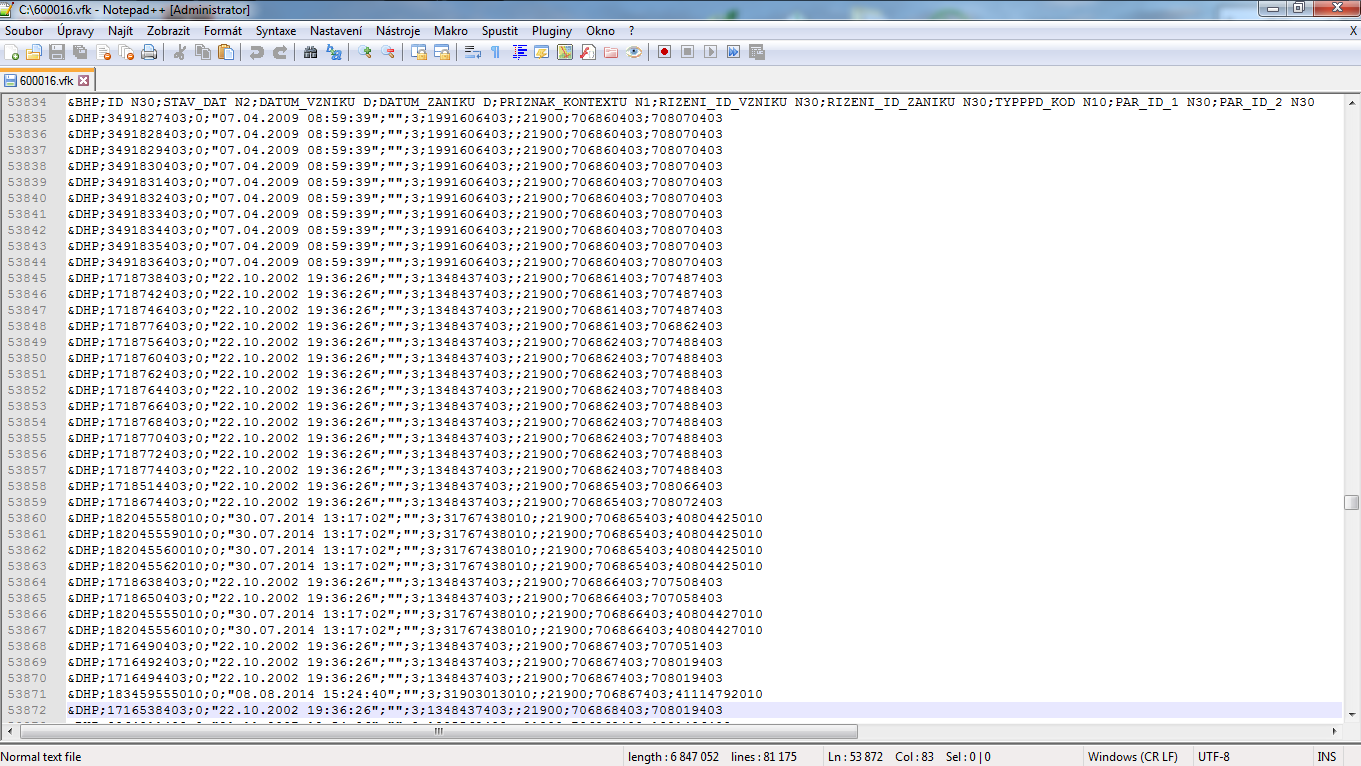
\includegraphics[width=15cm]{./pictures/testovaci_data.png}
      \caption{Ukázka bloku hranic parcel(HP) -- definice bloků a věty dat(zdroj:vlastní)}
      \label{fig:testovaci_data}
  \end{figure}
\begin{table}  
\caption{Ukázka bloku hranic parcel(HP) -- definice bloků a věty dat(zdroj:vlastní)}
\noindent\begin{tabular}{|p{\textwidth}|}
    \hline
    Zkouška vysázení \_ nebo třeba \% a co takhle \& to funguje? Zkouška vysázení \_ nebo třeba \% a co takhle \& to funguje? Zkouška vysázení \_ nebo třeba \% a co takhle \& to funguje?  \\ \hline
    Tak tohle už vypadá lépe: \_ nebo třeba \% \\ \hline
    kmenove\_cislo\_par \\ \hline
    \hline 
    \end{tabular}
\end{table}

\section{Výstupní data}
Výstupem k knihovny je sestavená geometrie pro bloky parcel a budov. Geometrie je společně s dalšími hodnotami jako je identifikační číslo, číslo parcely zapsána do vytvořené databáze.
\section{Popis tříd knihovny a jejich metod}
V této podkapitole budou představeny jednotlivé třídy knihovny, jejich členské metody a popsáno, co která třída a metoda obstarává.
\subsection{VFKBuilderError}
Tato třída dědí vlastnosti třídy Exception a je volána v případě, že nastane chyba. To se může stát není-li připojen \zk{VFK} souboru nebo databáze.
\subsection{VFKBuilder}
Mateřská třída, která obsahuje společné metody tříd VFKParBuilder a VFKBudBuilder určených pro sestavení geometrie parcel i budov.
\begin{itemize}
\item \verb|__init__()|
		
V konstruktoru třídy dochází k vytvoření tabulky geometrie (\verb|geometry columns|) a tabulky souřadného systému (\verb|spatial_ref_sys|), bez kterých by nebylo možné číst geometrii z databáze. V případě nepřipojeného zdroje dat - \zk{VFK} souboru, je volána třída VFKBuilderError a zobrazena chybová hláška.
\item \verb|build_bound()|

Jedna z hlavních metod, která sestavuje geometrii jednotlivých hranic. V případě hranice s dírami dojde k vytvoří seznamu s více geometriemi, ve kterém je nalezena největší a ze zbylých geometrií jsou vytvořeny díry. Sestavení probíhá geometrickou cestou. Nejdříve je přidána první hranice, poté hranice co začíná koncovým bodem první hranice a tak dokola. Na závěr je otestováno uzavření všech hranic v seznamu geometrií.
\item \verb|add_boundary()|

Metoda pro přidávání jedné hranice do geometrie. Přidávání hranice probíhá bod po bodu a přidaná hranice je ze seznamu hranic po přidání do geometrie odstraněna, aby se seznam zmenšil. Všechny hranice nemají stejnou orientaci(některé na sebe navazují koncovými body), tudíž je potřeba body hranice přidávat "odzadu".
\item \verb|get_sql_commands_from_file()|

Metoda otevírající soubor a vracející seznam SQL příkazů.
\item \verb|add_tables()|

Provádí příkazy, které dostane z metody \verb|get_sql_commands_from_file()|. Po ukončení cyklu s SQL příkazy je třeba zavolat metodu \textit{commit()} jinak nedojde z provedení posledního příkazu. Příkazy probíhají interně v transakci, kterou je třeba pro správné provedení ukončit.
\end{itemize}
\subsection{VFKBudBuilder}
Potomek třídy \textbf{VFKBuilder}. Třída sestavuje geometrii budov a ukládá ji do nově vytvořené tabulky BUD v databázi. Ukládání probíhá v transakci.
\begin{itemize}
\item \verb|__init__()|

Konstruktor třídy, kde je vytvořena nová tabulka pro budovy -- BUD a atribut \verb|id_bud|.
\item \verb|get_bud_id()|

SQL dotazem zjistí unikátní seznam identifikačních čísel budov. Dále vytvoří list, do kterého uloží seznamy s identifikačními čísly bodů pro každou budovu zvlášť.
\item \verb|filter_sbp()|

Na základě identifikačního čísla budovy najde všechny hranice, které k dané budově patří a vrací je uložené v seznamu. Volána třída VFKBuilderError v případě nepřipojené databáze.
\item \verb|build_all_bud()|

Zde probíhá samotné sestavení všech budov. Po sestavení je budova uložena do databáze i s příslušnými atributy. Metodě je možné nastavit kolik budov má sestavit. Základně dochází k sestavení všech budov.
\end{itemize}
\subsection{VFKParBuilder}
Potomek třídy \textbf{VFKBuillder}. V této třídě dochází k samotnému sestavení geometrie parcel, vytvoření nové tabulky PAR v databázi a zapsání dat. Zapisuje se identifikační číslo parcely(\verb|par_id|), kmenové číslo parcely(\verb|kmenove_cislo_par|), poddělení čísla parcely(\verb|poddeleni_cisla_par|) a samozřejmě geometrie dané parcely. Zápis do databáze je proveden v transakci, čímž je zaručené korektní zapsání všech parcel nebo žádné -- v případě chyby.

\begin{itemize}
\item \verb|__init__()|

Konstruktor třídy, kde je vytvořena nová tabulka pro parcely -- PAR včetně atributů.
\item \verb|get_par()|
		
Tato metoda vrací seznam unikátních identifikačních čísel parcel, který získá SQL dotazem, ve formátu seznamu. Volána třída VFKBuilderError v případě nepřipojené databáze.
\item \verb|filter_hp()|

Na základě identifikačního čísla parcely najde všechny hranice, které k dané parcele patří a vrací je uložené v seznamu. Volána třída VFKBuilderError v případě nepřipojené databáze.
\item \verb|build_all_par()|

Zde probíhá samotné sestavení všech parcel. Po sestavení je parcela uložena do databáze i s příslušnými atributy. Metodě je možné nastavit kolik parcel má sestavit. Základně dochází k sestavení všech parcel.

\end{itemize}
\section{Integrace knihovny}
Základem integrace bylo správné umístění do kódu zásuvného modulu. Bylo potřeba zachovat funkcionalitu při otevření úplných i neúplných dat. Jsou-li data úplná, funguje zásuvný modul standardně. Pokud data neobsahují bloky PAR a BUD -- jsou neúplná, dojde k jejich sestavení a tedy zavolání třídy z nově integrované knihovny \textbf{publicvfk}.

Nejdříve je knihovna pomocí metody import nahrána. Dále je ve funkci \textbf{loadVfkFile()} proveden test na přítomnost bloku parcel('PAR') pomocí metody GetLayerName():

\verb|t_par = self.__mOgrDataSource.GetLayerByName('PAR')|
Předpokladem je, že bloky parcel a budov jsou v datech oba nebo žádný, proto je testována jen přítomnost bloku parcel. Není-li blok obsažen, dojde k uzavření zdroje dat:

\verb|self.__mOgrDataSource = None|
, aby mohlo proběhnout sestavení bloků. Knihovna si vytváří vlastní připojení k \zk{VFK} souboru a databázi, proto je třeba zdroj dat uzavřít a předejít tak zdvojenému připojení. Následuje sestavení neobsažených bloků:

\verb|# Build Parcels|

\verb|parcels = VFKParBuilder(fileName)|

\verb|parcels.build_all_par()|

\verb|# Build Buildings|

\verb|buildings = VFKBudBuilder(fileName)|

\verb|#buildings.build_all_bud()|

Po sestavení bloků parcel a budov je zdroj dat pomocí proměnné prostředí nastaven na databázi, která vznikne o adresář dřív při otevření \zk{VFK} souboru a nese jméno \zk{VFK} souboru, kde je místo přípony \verb|_stav.db|:

\verb|self.__mOgrDataSource = ogr.Open(os.environ['OGR_VFK_DB_NAME'], 0)|

\verb|self.__mDataSourceName = os.environ['OGR_VFK_DB_NAME']| %proc nastavuje zde taky prostredi?

V této databázi jsou uložena data z načtení \zk{VFK} souboru a také knihovnou vytvořené tabulky s bloky PAR a BUD.
\section{Testování knihovny}
Funkčnost knihovny je možné otestovat z příkazové řádky. K testování byl využit modul sys, který je obsažen v základní distribuci Pythonu a díky kterému je možné realizovat množství úloh spojených s interpretrem. Příkaz pro spuštění se skládá z názvů knihovny a vfk souboru včetně přípony, oddělených mezerou. Například: python publicvfk.py 600016.vfk. Jméno knihovny a další argumenty(v našem případě název vfk souboru) předané z příkazové řádky jsou uloženy v proměnné \textit{sys.argv}.

Pokud není zadán název knihovny i název vfk souboru, je interpretr ukončen a zobrazena chybová hláška.
    %if len(sys.argv) != 2:
        %sys.exit("{} soubor.vfk".format(sys.argv[0]))

Testování je možné jen při přímém spuštění knihovny, nikoli je-li knihovna importována jako modul. K tomu je využita speciální proměnná \verb|__name__|, do které je interpretrem v případě spuštění přímo uložena hodnota \verb|"__main__"| a podmínka je splněna. Je-li knihovna importována z jiného modulu je proměnná \verb|__name__| nastavena na jméno modulu a podmínka není splněna.
 
%if __name__ == "__main__":
%ucebnice jazyka Python str 10